\documentclass[11pt]{article}
\usepackage{graphicx}
\usepackage[english]{babel}
\usepackage{amsmath}
\usepackage[section]{placeins}
\graphicspath{ {./images/} }

\usepackage[T1]{fontenc}
\usepackage{listings}
\usepackage{hyperref}
\usepackage{color}

\definecolor{dkgreen}{rgb}{0,0.6,0}
\definecolor{gray}{rgb}{0.5,0.5,0.5}
\definecolor{mauve}{rgb}{0.58,0,0.82}

\lstset{frame=tb,
  language=C++,
  aboveskip=3mm,
  belowskip=3mm,
  showstringspaces=false,
  columns=flexible,
  basicstyle={\small\ttfamily},
  numbers=none,
  numberstyle=\tiny\color{gray},
  keywordstyle=\color{blue},
  commentstyle=\color{dkgreen},
  stringstyle=\color{mauve},
  breaklines=true,
  breakatwhitespace=true,
  tabsize=3
}

\setlength{\parindent}{0pt}
\setlength{\parskip}{0pt plus 0.5ex}
%% adjust spacing for all itemize/enumerate

\begin{document}


\tableofcontents

% TODO: add in more links whenever possible
\section{Useful Resources}
Robot modelling in urdf is rather tedious. Here are a couple of guides/tips which I have found useful.


\begin{itemize}
 \item {
       \href{https://nu-msr.github.io/me495_site/lecture06_modeling.html}{URDF/xacro guide}
       }
 \item{
       \href{   https://classic.gazebosim.org/tutorials?tut=ros_gzplugins}{Guide for gazebo plugins (used to simulate sensors/actuators in gazebo)}
       }
 \item{
       \href{
        https://medium.com/teamarimac/integrating-sonar-and-ir-sensor-plugin-to-robot-model-in-gazebo-with-ros-656fd9452607
       }{Sonar Plugin Guide}
       }
 \item{
       This is a folder which contains many gazebo .world files.
       \begin{lstlisting}[language=bash]
        /usr/share/gazebo-9/worlds
       \end{lstlisting}
       }
       
\end{itemize}
\section{Useful Tools}
\begin{itemize}
 \item {Fusion 360 - A CAD software. Quite useful for measuring the dimensions of mesh files }
 \item { Mesh Lab - A piece of software to visualise and manipulate mesh files.}
\end{itemize}


\section{Installation}
\begin{enumerate}
 \item{Install the joint state publisher:
       \begin{lstlisting}[language=bash]
$ sudo apt install ros-melodic-joint-state-publisher-gui
       \end{lstlisting}
       }
 \item{
       Next, git clone realsense package into your catkin/src folder.
       
       \begin{lstlisting}[language=bash]
$ git clone https://github.com/SynapseProgramming/realsense_gazebo_plugin.git
       \end{lstlisting}
       }
       
 \item{
       % https://github.com/SynapseProgramming/map2gazebo.git
       Next, git clone the map2gazebo package into your catkin/src folder
       
       \begin{lstlisting}[language=bash]
$ git clone https://github.com/SynapseProgramming/map2gazebo.git
       \end{lstlisting}
       }
       
       
 \item{
       Enter the following command into the terminal to setup gazebo environment variables
       \begin{lstlisting}[language=bash]
       $ echo "source /usr/share/gazebo/setup.sh" >> ~/.bashrc
       $ source ~/.bashrc
       \end{lstlisting}
       
       }
 \item{
       Lastly, remember to run the cakin\_make command.
       }
       
       % TODO: add in the fake_world package once done.
       % add back the excluded stl mesh files.
       % not sure if this package should be stored in gitlab or gitub
\end{enumerate}

\section{Package Overview}
\subsection{world}
The world folder is used to store gazebo .world files. .world files are used to describe the surrounding environment in Gazebo.
\subsection{urdf}
The urdf folder is used to store (.urdf.xacro) and (.gazebo.xacro) files.
\begin{itemize}
 \item {
       (.urdf.xacro) files describe the transformations between the various links of the robot, along with other variables such as intertia.
       }
 \item{
       (.gazebo.xacro) files would describe the kinematic properties of the robot such as velocity limits, coefficient of friction etc.
       }
\end{itemize}
\subsubsection{Intel Realsense D435 camera}
\begin{itemize}
 \item {
       The (\_d435.gazebo.xacro) file is used to describe the various kinematic properties of the depth camera.
       }
 \item{
       The (\_d435.urdf.xacro) file is used to describe the various frames of the depth camera.
       
       The (<camera>\_bottom\_screw\_frame) is used as the main reference point for the depth camera. It is centered about the bottom tripod mount of the depth camera.
       Thus, to define the position of the depth camera on the robot, we would have to provide the transformation from base link to the bottom screw frame link
       }
\end{itemize}

\subsection{meshes}
The meshes folder is used to store the various mesh files of the robot(.stl .dae).
The mesh files are used to visualize various components of the robot(sensors, chassis) and to enable accurate collisions within gazebo.

\subsection{rviz}
The rviz folder is used to store the various rviz configs.

% TODO: update launch section when more launch files are created
\subsection{launch}
\begin{itemize}
 \item{
       
       The launch folder is used to store roslaunch files. Launch files titled simulate\_<robotname>.launch are used to launch the gazebo simulation environment and rviz.
       }
 \item{
       Launch files titled view\_<robot>.launch are used to view the robots urdf model in rviz.
       }
\end{itemize}


% TODO: complete the section on how to scale and manipulate stl files so that the mesh could be easily integrated into rviz

\section{Mesh Manipulation}
\subsection{Reducing the quality of a mesh (Mesh Lab)}
In most cases, the generated meshes are too large for gazebo to render at a high framerate. Thus, we would have to reduce the resolution of our meshes.
\begin{enumerate}
 \item {
       Open meshlab and import the mesh (file > import mesh)
       }
 \item{
       Click on Filters > Remeshing, Simplification and Reconstruction >  Quadratic edge collapse decimation
       }
 \item{
       Select a lower number of (target number of faces) and click apply.
       }
 \item{
       click on file > export mesh as > (enter mesh name and select \emph{.stl} file type)
       }
\end{enumerate}
\subsection{Scaling Down a mesh (Fusion 360) }
\begin{enumerate}
 \item {
       Click on insert > insert mesh
       }
 \item {
       Select the correct units for the given mesh and select center position.
       }
 \item {
       Click on mesh > modify > scale mesh
       }
 \item {
       Click on the mesh and apply a scale factor of 0.1
       }
 \item {
       Repeat steps 3 and 4 repeatedly until the desired scale factor is achieved (for example, this process would have to be repeated 3 times to scale from \emph{mm} to \emph{m} )
       }
 \item{
       Save the project, and export the final mesh as a .stl file.
       }
\end{enumerate}

\subsection{Mesh Origin}
Each stl file has a origin. In most cases, we would want to modify the origin for various reasons.

\subsubsection{Centering a mesh}
\begin{enumerate}
 \item {
       Import a mesh into meshlab.
       }
 \item{
       click on render > show axis
       }
 \item{
       click on filters > Normals Curvature and Orientation > Transform: Move, Translate, Center
       }
 \item{
       Select translate center of bbox to the origin and click apply.
       
       }
       
\end{enumerate}
\emph{In most cases, the centered origin is used to as the centre of mass. Thus, intertia is computed with respect to the centered origin.}
\subsubsection{Translating \& rotating a mesh}
\begin{itemize}
 \item {
       Under filters > Normals Curvature and Orientation, there are a few transform operations which could carried out on the mesh.
       }
\end{itemize}

\emph{Do take note of the translation between the center origin of the mesh, and the final origin of the mesh as we would have to take that into account when defining the intertia reference frame.}
\section{Computing Intertia of meshes}
In Gazebo, the inertia parameters should be well defined as they are used by the physics engine.
Incorrect inertia parameters may result in odd occurences such as sliding on the spot.
\subsection{Key Variables}
\begin{itemize}
 \item {
       scaling factor $s$
       \begin{itemize}
        \item {URDF uses $m$ (metres) to measure distance.}
        \item{ Most \emph{.stl} files would be in $mm$ (milimetres) }
        \item{In this example, scaling factor $s=10^2$ (the .stl file is in $cm$)}
       \end{itemize}
       }
 \item{
       Mesh Origin
       
       The center origin of the mesh would be used as the reference frame for intertia.
       
       Therefore, if the center origin of the mesh is not used as the main origin for the current part, we would have to
       specify the translation from the main origin to the center origin.
       
       
       \begin{figure}[!htb]
        \centering
        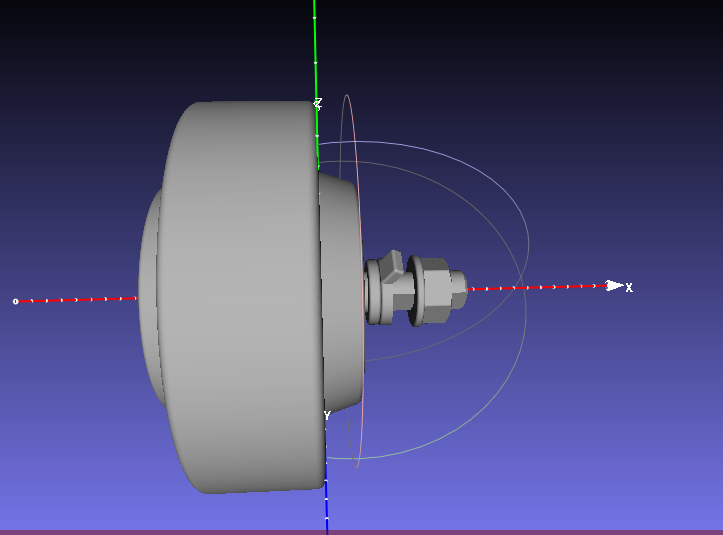
\includegraphics[width=0.5\textwidth]{images/centeredwheel}
        \caption{Wheel mesh with centered origin}
       \end{figure}
       
       
       \begin{figure}[!htb]
        \centering
        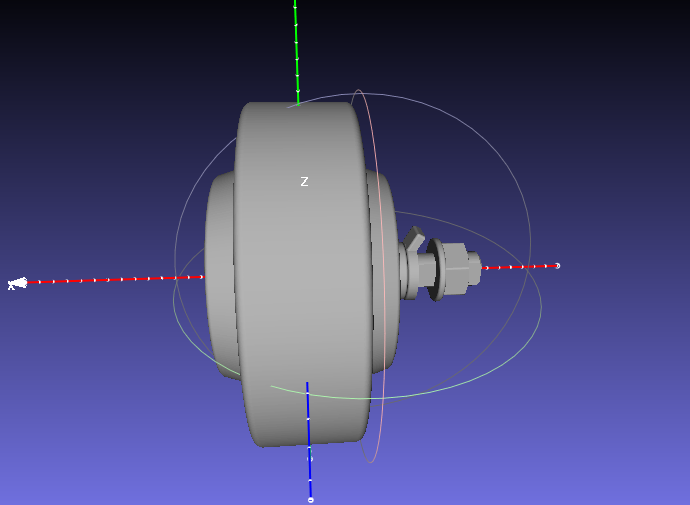
\includegraphics[width=0.5\textwidth]{images/offcenteredwheel}
        \caption{Wheel mesh with off-centered origin}
       \end{figure}
       }
\end{itemize}
\subsection{Computing Intertia }
\begin{enumerate}
 \item {Firstly, import the mesh into meshlab.}
 \item{Ensure that the current origin of the mesh is its center.}
 \item{ Click on filters > Cleaning and Repairing > Remove Duplicate Faces}
 \item{ Click on view > Show Layer Dialog (ensure that a right window pops up)}
 \item {Click on filters > Quality measure and computations > Compute Geometric Measures}
 \item {
       At the bottom right corner, the following text would be generated.
       \begin{lstlisting}[language=bash]

        Mesh Bounding Box Size 10.275001 13.000000 13.000000
        Mesh Bounding Box Diag 21.061235
        Mesh Volume is 575.673584
        Mesh Surface is 1340.176147
        Thin shell barycenter -0.288410 0.036296 0.007559
        Center of Mass is -0.142327 0.002174 0.000383
        Inertia Tensor is :
        | 10287.553711 2.708627 0.324480 |
        | 2.708627 6752.031738 -0.408094 |
        | 0.324480 -0.408094 6754.208984 |
        Principal axes are :
        | 1.000000 -0.000770 0.000046 |
        | 0.000766 0.983973 -0.178316 |
        | 0.000092 0.178316 0.983973 |
        axis momenta are :
        | 10287.555664 6751.955566 6754.282715 |

       \end{lstlisting}
       \begin{itemize}
        \item {
              The Intertia Tensor generated by MeshLab would correspond to the following matrix
              $$
               \begin{bmatrix}
                I_{xx} & I_{xy} & I_{xz} \\
                I_{xy} & I_{yy} & I_{yz} \\
                I_{xz} & I_{yz} & I_{zz} \\
               \end{bmatrix}
              $$
              }
        \item{
              As the mesh used in this example is in $cm$, the mesh volume would be in ${cm}^3$
              }
       \end{itemize}
       
       }
\end{enumerate}
\subsection{Importing Inertia Values into URDF}
\begin{enumerate}
 \item {
       
       Each element in the inertia matrix would have to be scaled down by $s^5$, where $s$ is the scaling factor.
       (eg. s=$10^2$ for a mesh in $cm$. Thus, each $I$ value would have to be multiplied by $10^{-10}$)
       
       $$
        \frac{1}{s^5}
        \begin{bmatrix}
         I_{xx} & I_{xy} & I_{xz} \\
         I_{xy} & I_{yy} & I_{yz} \\
         I_{xz} & I_{yz} & I_{zz} \\
        \end{bmatrix}
       $$
       }
 \item{
       As the generated mesh volume is in ${cm}^3$, we would have to multiply the mesh volume by $10^{-6}$ to scale it to $m^3$.
       }
 \item{
       Lastly, we would have to fill up the inertia tag in the URDF file.
       \begin{itemize}
        \item { \emph{origin} tag should be filled with the translation from the main origin to the center origin (if neccessary)}
        \item { \emph{inertia} tag should be filled with the scaled inertia values. }
        \item { \emph{mass} tag should be filled with the scaled mesh volume (meshlab assumes a density of 1).}
       \end{itemize}
       \begin{lstlisting}[language=bash]
    <inertial>
      <origin xyz="0 0 0"/>
      <mass value="575.673584e-6"/>
      <inertia ixx="10287.553711e-10" ixy="2.708637e-10" ixz="0.324480e-10" iyy="6752.031738e-10" iyz="-0.408100e-10" izz="6754.208984e-10"/>
    </inertial>

       \end{lstlisting}
       
       
       }
\end{enumerate}
\subsection{Verifying Inertia Values}
If the inertia values were computed correctly, then the mesh should have a pink box surrounding the mesh in Gazebo (view > inertia)
\begin{figure}[!h]
 \centering
 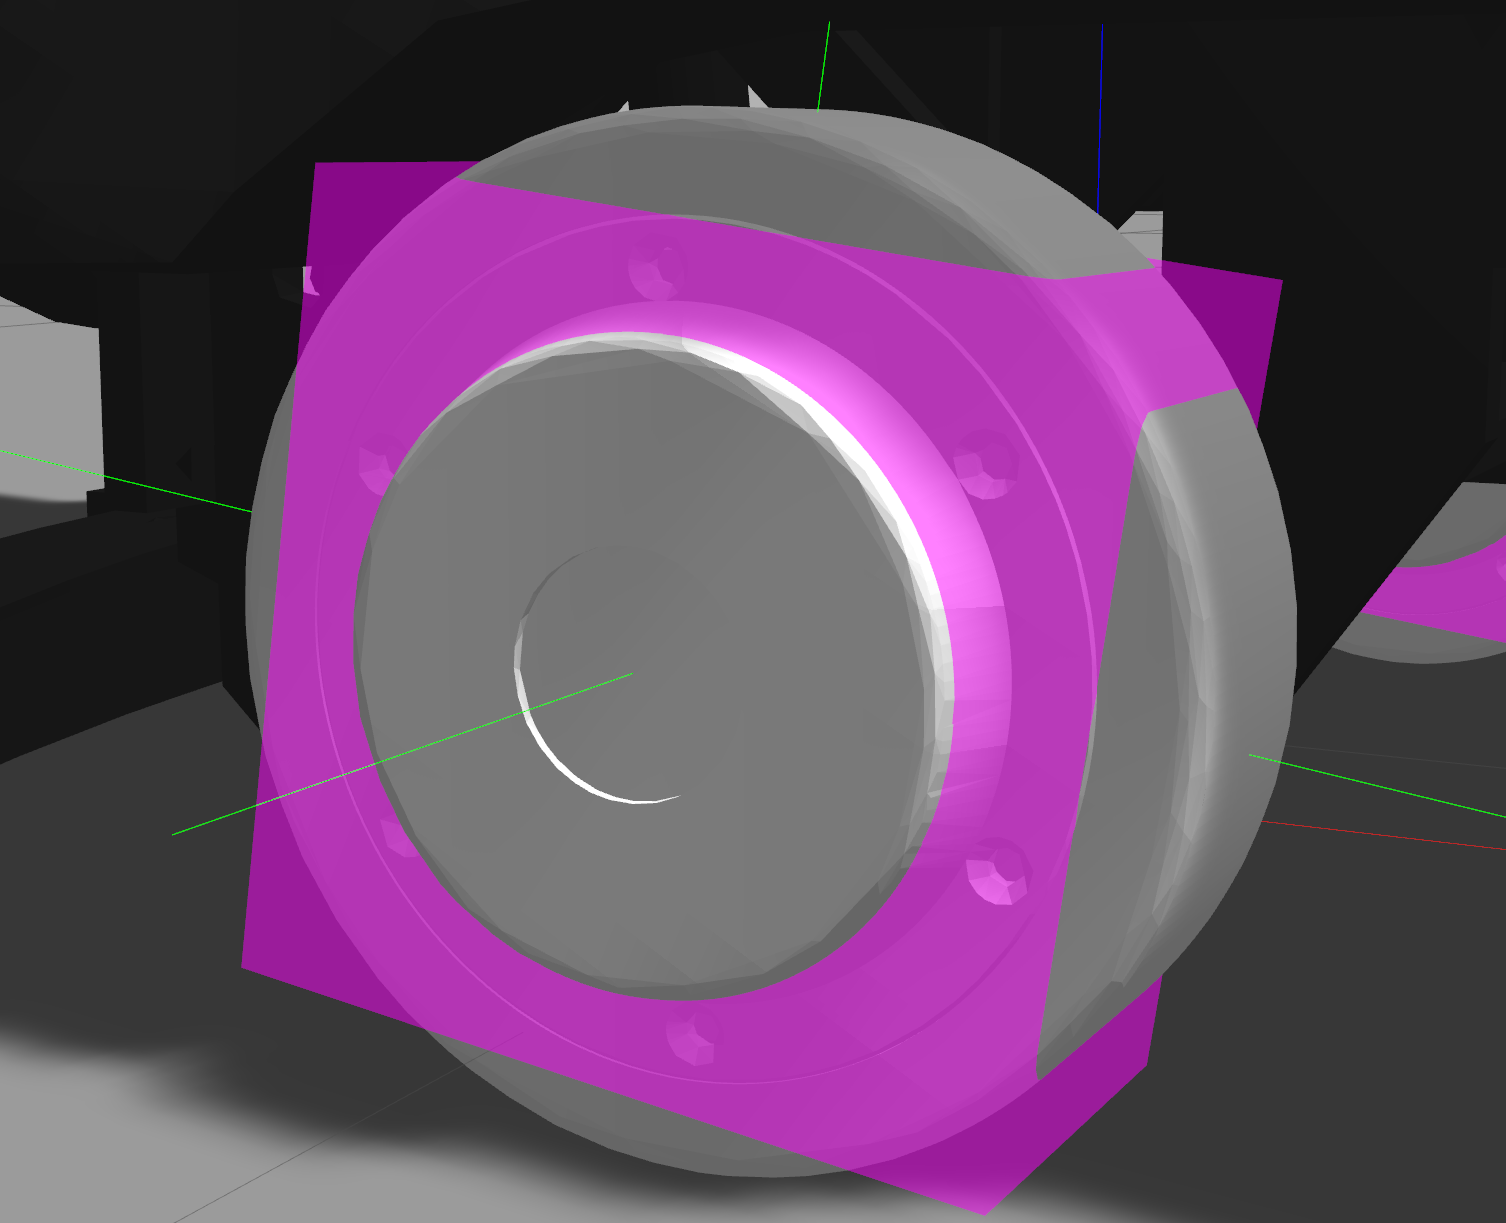
\includegraphics[width=0.5\textwidth]{images/inertiawheel}
 \caption{Wheel with inertia bounding box}
\end{figure}

\section{Gazebo World from 2D Map}
\subsection{Setup \& Installation}

\begin{enumerate}
 \item{
       Ensure that the map server is installed on your system.
       \begin{lstlisting}[language=bash]
     $ sudo apt install ros-melodic-map-server
       \end{lstlisting}
       }
 \item{
       Clone the \href{https://github.com/SynapseProgramming/map2gazebo.git
       }{\emph{map2gazebo}} repository into your catkin/src folder.
       
       }
 \item{
       Navigate to the \emph{map2gazebo} package in your catkin/src folder and run the following commands.
       
       \begin{lstlisting}[language=bash]
         $ pip install --user trimesh
         $ pip install --user numpy
         $ pip install --user pycollada
         $ pip install --user scipy
         $ pip install --user networkx
       \end{lstlisting}
       }
 \item{
       Lastly, navigate to your catkin\_ws folder and run catkin\_make
       }
\end{enumerate}

\subsection{Generation of map.stl file}

\begin{enumerate}
 \item{launch roscore}
 \item {
       Navigate to the folder containing the \emph{pgm} and \emph{yaml} file for the map that you would want to convert and run the following command to launch the map server.
       \begin{lstlisting}[language=bash]
        $ rosrun map_server map_server <map name>.yaml
       \end{lstlisting}
       }
 \item{
       Then, run the following command to generate the \emph{map.stl} at a given directory. (replace
       \emph{/home/roald/Desktop/generatedmaps} with your own path)
       
       \begin{lstlisting}[language=bash]
        $ roslaunch map2gazebo map2gazebo.launch export_dir:=/home/roald/Desktop/generatedmaps
        \end{lstlisting}
       }
\end{enumerate}
\subsection{Importing the mesh into Gazebo}
\begin{enumerate}
 \item {
       Firstly, navigate to the following directory
       \begin{lstlisting}[language=bash]
 catkin_ws/src/map2gazebo/models/map/meshes
        \end{lstlisting}
       }
 \item {
       Replace the existing map.stl file with the newly generated map.stl file.
       }
 \item{
       Launch the following command to launch the gazebo simulation with the current robot in the new map.
       \begin{lstlisting}[language=bash]
       $ roslaunch fake_world simulate_cub_lab.launch
        \end{lstlisting}
       
       }
\end{enumerate}

\section{multimaster\_fkie}
Multimaster\_fkie is a collection of packages which allows topics to be passed between separate devices, while running separate masters.


\subsection{Networking}
\begin{itemize}
 \item { All machines should be connected to the same local network}
 \item{ DHCP reservation could be used to ensure that the machines have a static IP address}
\end{itemize}
\subsection{Package Installation }
\begin{enumerate}
 \item {
       Enter the following lines to install the package dependencies.
       \begin{lstlisting}[language=bash]
       $ sudo add-apt-repository ppa:roehling/grpc
       $ sudo apt update
       $ sudo apt install python-grpcio python-grpc-tools
        \end{lstlisting}
       }
 \item{
       Next, navigate to your catkin/src folder and run the following command.
       \begin{lstlisting}[language=bash]
         $ git clone https://github.com/fkie/multimaster_fkie.git
        \end{lstlisting}
       }
 \item{
       Lastly, run catkin\_make to build the package.
       }
       % roslaunch fkie_master_discovery master_discovery.launch
\end{enumerate}
\subsection{Setup \& Usage}

In this section, we shall assume that we would want to pass data between two machines, \emph{M1} and \emph{M2}.

\begin{enumerate}
 \item {
       Ensure that the multimaster\_fkie package is installed on both machines.
       }
 \item {
       Ensure that only one networking option is enabled (either wifi or ethernet)
       }
 \item{
       Next, run the \emph{ifconfig} command on \emph{M1} and \emph{M2} and note down the  assigned ip address.
       }
 \item{
       Next, navigate to the \emph{etc} directory and run the following command
       \begin{lstlisting}[language=bash]
        $ sudo gedit hosts
        \end{lstlisting}
       }
 \item{
       Add the ip addresses of M1 and M2 to the hosts file (replace the fake ip-addresses with real ones and replace \emph{M1} and \emph{M2} with the names of your machines)
       
       (example hosts file for \emph{M1})
       \begin{lstlisting}[language=bash]
       127.0.0.1 localhost
       127.0.1.1 M1

       #for ROS multimaster
       12.13.14.15 M1
       14.13.153.134 M2
        \end{lstlisting}
       }
 \item{
       Repeat steps 3 and 4 on  the other machine. (eg. \emph{M2})
       }
 \item{
       Ensure that roscore is running on both machines \emph{M1} and \emph{M2}
       }
 \item{
       Run the following commands in separate terminals to sync up the two rosmasters on \emph{M1} and \emph{M2}
       \begin{lstlisting}[language=bash]
         $ rosrun fkie_master_discovery master_discovery
         $ roslaunch fkie_master_sync master_sync.launch
        \end{lstlisting}
       
       }
\end{enumerate}
\subsection{Testing}
\begin{enumerate}
 \item {
       Firstly, ensure that roscore, the discovery and the master sync nodes are running on both machines \emph{M1} and \emph{M2}.
       }
 \item{
       Next, run the following command to check if both masters are known by the discovery node.
       Ideally, both masters on the separate machines should be listed here.
       \begin{lstlisting}[language=bash]
         $ rosservice call /master_discovery/list_masters
        \end{lstlisting}
       }
 \item{
       Next, run the following command in \emph{M1} to run the turtlesim node.
       \begin{lstlisting}[language=bash]
          $ rosrun turtlesim turtlesim_node
        \end{lstlisting}
       }
 \item{
       Next, run the following command in \emph{M2} to run the turtlesim teleop node.
       \begin{lstlisting}[language=bash]
          $ rosrun turtlesim turtle_teleop_key
        \end{lstlisting}
       }
 \item{
       Thus, if all went well, pressing the arrow keys on \emph{M2} should move the turtle on \emph{M1}.
       }
\end{enumerate}
\section{Gzweb}
\subsection{Setup \& Installation}
\begin{enumerate}
 \item {
       Firstly, open a new terminal and enter the following commands.
       you may wish to refer to \href{https://classic.gazebosim.org/tutorials?tut=gzweb_install&cat=gzweb}{\emph{this gazebo webpage}}
       \begin{lstlisting}[language=bash]
$ sudo apt install gazebo9 libgazebo9-dev
$ sudo apt install libjansson-dev libboost-dev imagemagick libtinyxml-dev mercurial cmake build-essential
$ curl -o- https://raw.githubusercontent.com/nvm-sh/nvm/v0.35.3/install.sh | bash
$ source ~/.bashrc
$ nvm install 8
$ cd ~; git clone https://github.com/osrf/gzweb
$ cd ~/gzweb
$ git checkout gzweb_1.4.1
$ npm run deploy --- -m
       \end{lstlisting}
       }
 \item{
       Next, navigate to the
       gzweb/http/client/assets
       directory and copy and paste the fake\_world package in the assets directory.
       }
 \item { Navigate to the gzweb directory and run \emph{npm install}}
\end{enumerate}
\subsection{Usage}
\begin{enumerate}

 \item { Navigate to the gzweb directory and run \emph{npm start}}
 \item{
       Lastly, ensure that the launch file in the simulation package has the GUI tag disabled, before proceeding to enter the roslaunch command.
       \begin{lstlisting}[language=bash]
          <arg name="gui" value="false"/>
       \end{lstlisting}
       }
\end{enumerate}

\end{document}
